\subsection{Previous writing}

For the Sea Ice Charts, ice charts from the bulletin date and valid date are selected. From AA, relevant meteorological fields are selected and daily means are computed (more details in following sections). Finally, from OSI-SAF a sea ice trend is computed. For a given bulletin date, the data fetched above is stored in a .hdf5 file, such that each sample (bulletin date) is represented by its own .hdf5 file. Furthermore, a dataloader object is initialized with a list of .hdf5 files, with the list containing filenames of the samples constituting a data subset such as train, validation or test data. This processes is visualized in Figure (\ref{fig:pipeline_sketch}).


\subsection{Data sources}
Data sources used are Sea Ice charts from Nick initiated at 15:00 as well as Arome Arctic initiated at 18:00 \cite{Dinessen2020,Mueller2017}. For a given date, the current Ice Chart is used as a predictor for the model, while the Ice Chart drawn two days later is supplied as the model target.

\subsubsection{Sea Ice Charts}
The Sea Ice Charts used are a derived dataset of the Sea Ice Charts presented in a previous section \todo{label sections}. The present Ice Chart dataset has been postprocessed by Nick Hughes of the National Ice Service \todo{Say thanks in acknowledgements}, such that they are presented on a 1km Arome Arctic grid. Furthermore, the Ice Charts does not feature a land-mask, which has been replaced with interpolated values resulting in a spatially consistent dataset where all values present are according to the WMO Sea Ice Concentration intervals \cite{JETSI2014}. 

\subsection{AROME-Arctic}
The Arome Arctic data is structured such that the period between forecast initialization and machine learning forecast lead time is stored as a mean product in the temporal dimension at intervals [0 - 18, 42, 66]. This ensures that temporal AA information is encoded into a single field up until 12:00 UTC of the publishing date of the target ice chart. The 4d variables used from AA are T2M, uwind and vwind. Finally, the land sea mask present in AA is fetched and used as a predictor, though this land sea mask is also used for validation purposes given the case where no other SIC-product is considered.

\subsection{OSI-SAF}
\todo{Mention how when using Osi Saf trend as predictor, the trend up to but not including the forecast start date is used. This is to make the model ready for operational use, as the Osi Saf daily product is not ready on lustre when the Ice Charts are poublished at UTC 15:00}
A linear SIC trend of variable temporal length is computed from 12.5km OSI-SAF data \todo{Cite OSISAF}. In the case of OSI-SAF, the product is scheduled to be published daily at 15:00 UTC \todo{double check}. However, given operational concerns of the developed forecasting system, where the availability of data is essential for the model to run, the previous day OSI-SAF trend is utilized. \todo{Det er ikke sikkert det er nødvendig, hvis AA 18:00 publiseres ~19 - 20 burde OSI-SAF være publisert}.

OSI-SAF SSMIS is a continously developed operational product, where changes are not required to act retroactively on the data. As such, the Sea Ice Concentration used for few samples with t2m runs and many data samples no t2m differ due to the introduction of a filtered ice concentration variable 10/05-2017 \cite{Tonboe2017}. Thus, the filtered ice concentration will be used when the training data spans 2019-2020, and the unfiltered ice concentration will be used when the training data spans 2011 - 2018 to assert that there is no sudden shift in the ice concentration trend which can negatively impact the training period.


\subsection{Deviations from the U-Net}
% Although the U-Net formulation in Figure (\ref{fig:unet-overview}) applies a Stride $S = 1$, the current implementation also applies a zero padding $P = 1$ to the input which ensures that the shape of the output is equal to the input according to Equation (\ref{eq:outputdim}).

% Each activation is also proceeded by a normalization layer \citep{Ioffe2015,Wu2018} which has been customary in the field after their introduction in \citet{Ioffe2015} as they make the network converge towards a solution faster. 


% The intention of this section is currently to log the notes made during model development. What is written may be discussion like, and can thus be used as a basis for the actual thesis. However, this section is to be included in the final thesis.tex after extensive rewriting. Remember that good thesis work is well documented thesis work!

The model developed for the two day prediction is based on the SimpleUNET architecture, though with a different sized Input layer to accommodate for the changed dataloader. The dataloader has subsequently been changed to appropriately select the correct fields from the .hdf5 samples and appoint them as input or target variables. As a result of using three variables of two days mean AA forecast, as well as sst, land-sea-mask and current time-step ice chart, the total number of predictors fed into the model is 9. Moreover, the resolution of all fields are kept at 1km, though their spatial extent is limited to (1920 x 1840). This resolution and spatial size conserves (almost) the entirety of the west-east axis of the AA domain. However, the southern border is raised by 450km compared to the AA domain. There are two main motivations behind readjusting the spatial extent of the predictors and targets.

\begin{itemize}
    \item[1.] The spatial extent of the input domain has to be divisible by the reducing factor enforced by the MaxPooling operation performed in the encoding component of the UNET.
    \item[2.] The southern latitudes covered by AA has a proportionally skewed Sea Ice / Ice Free open water ratio, as exemplified in Figure (\ref{fig:exampleAAsouthborder}). Increasing the southern bounding latitude of the subdomain thus decreases the number of guaranteed ice free pixels, which in turn decreases the skewness towards the ice free open water class for the UNET.
\end{itemize}

\begin{figure}
    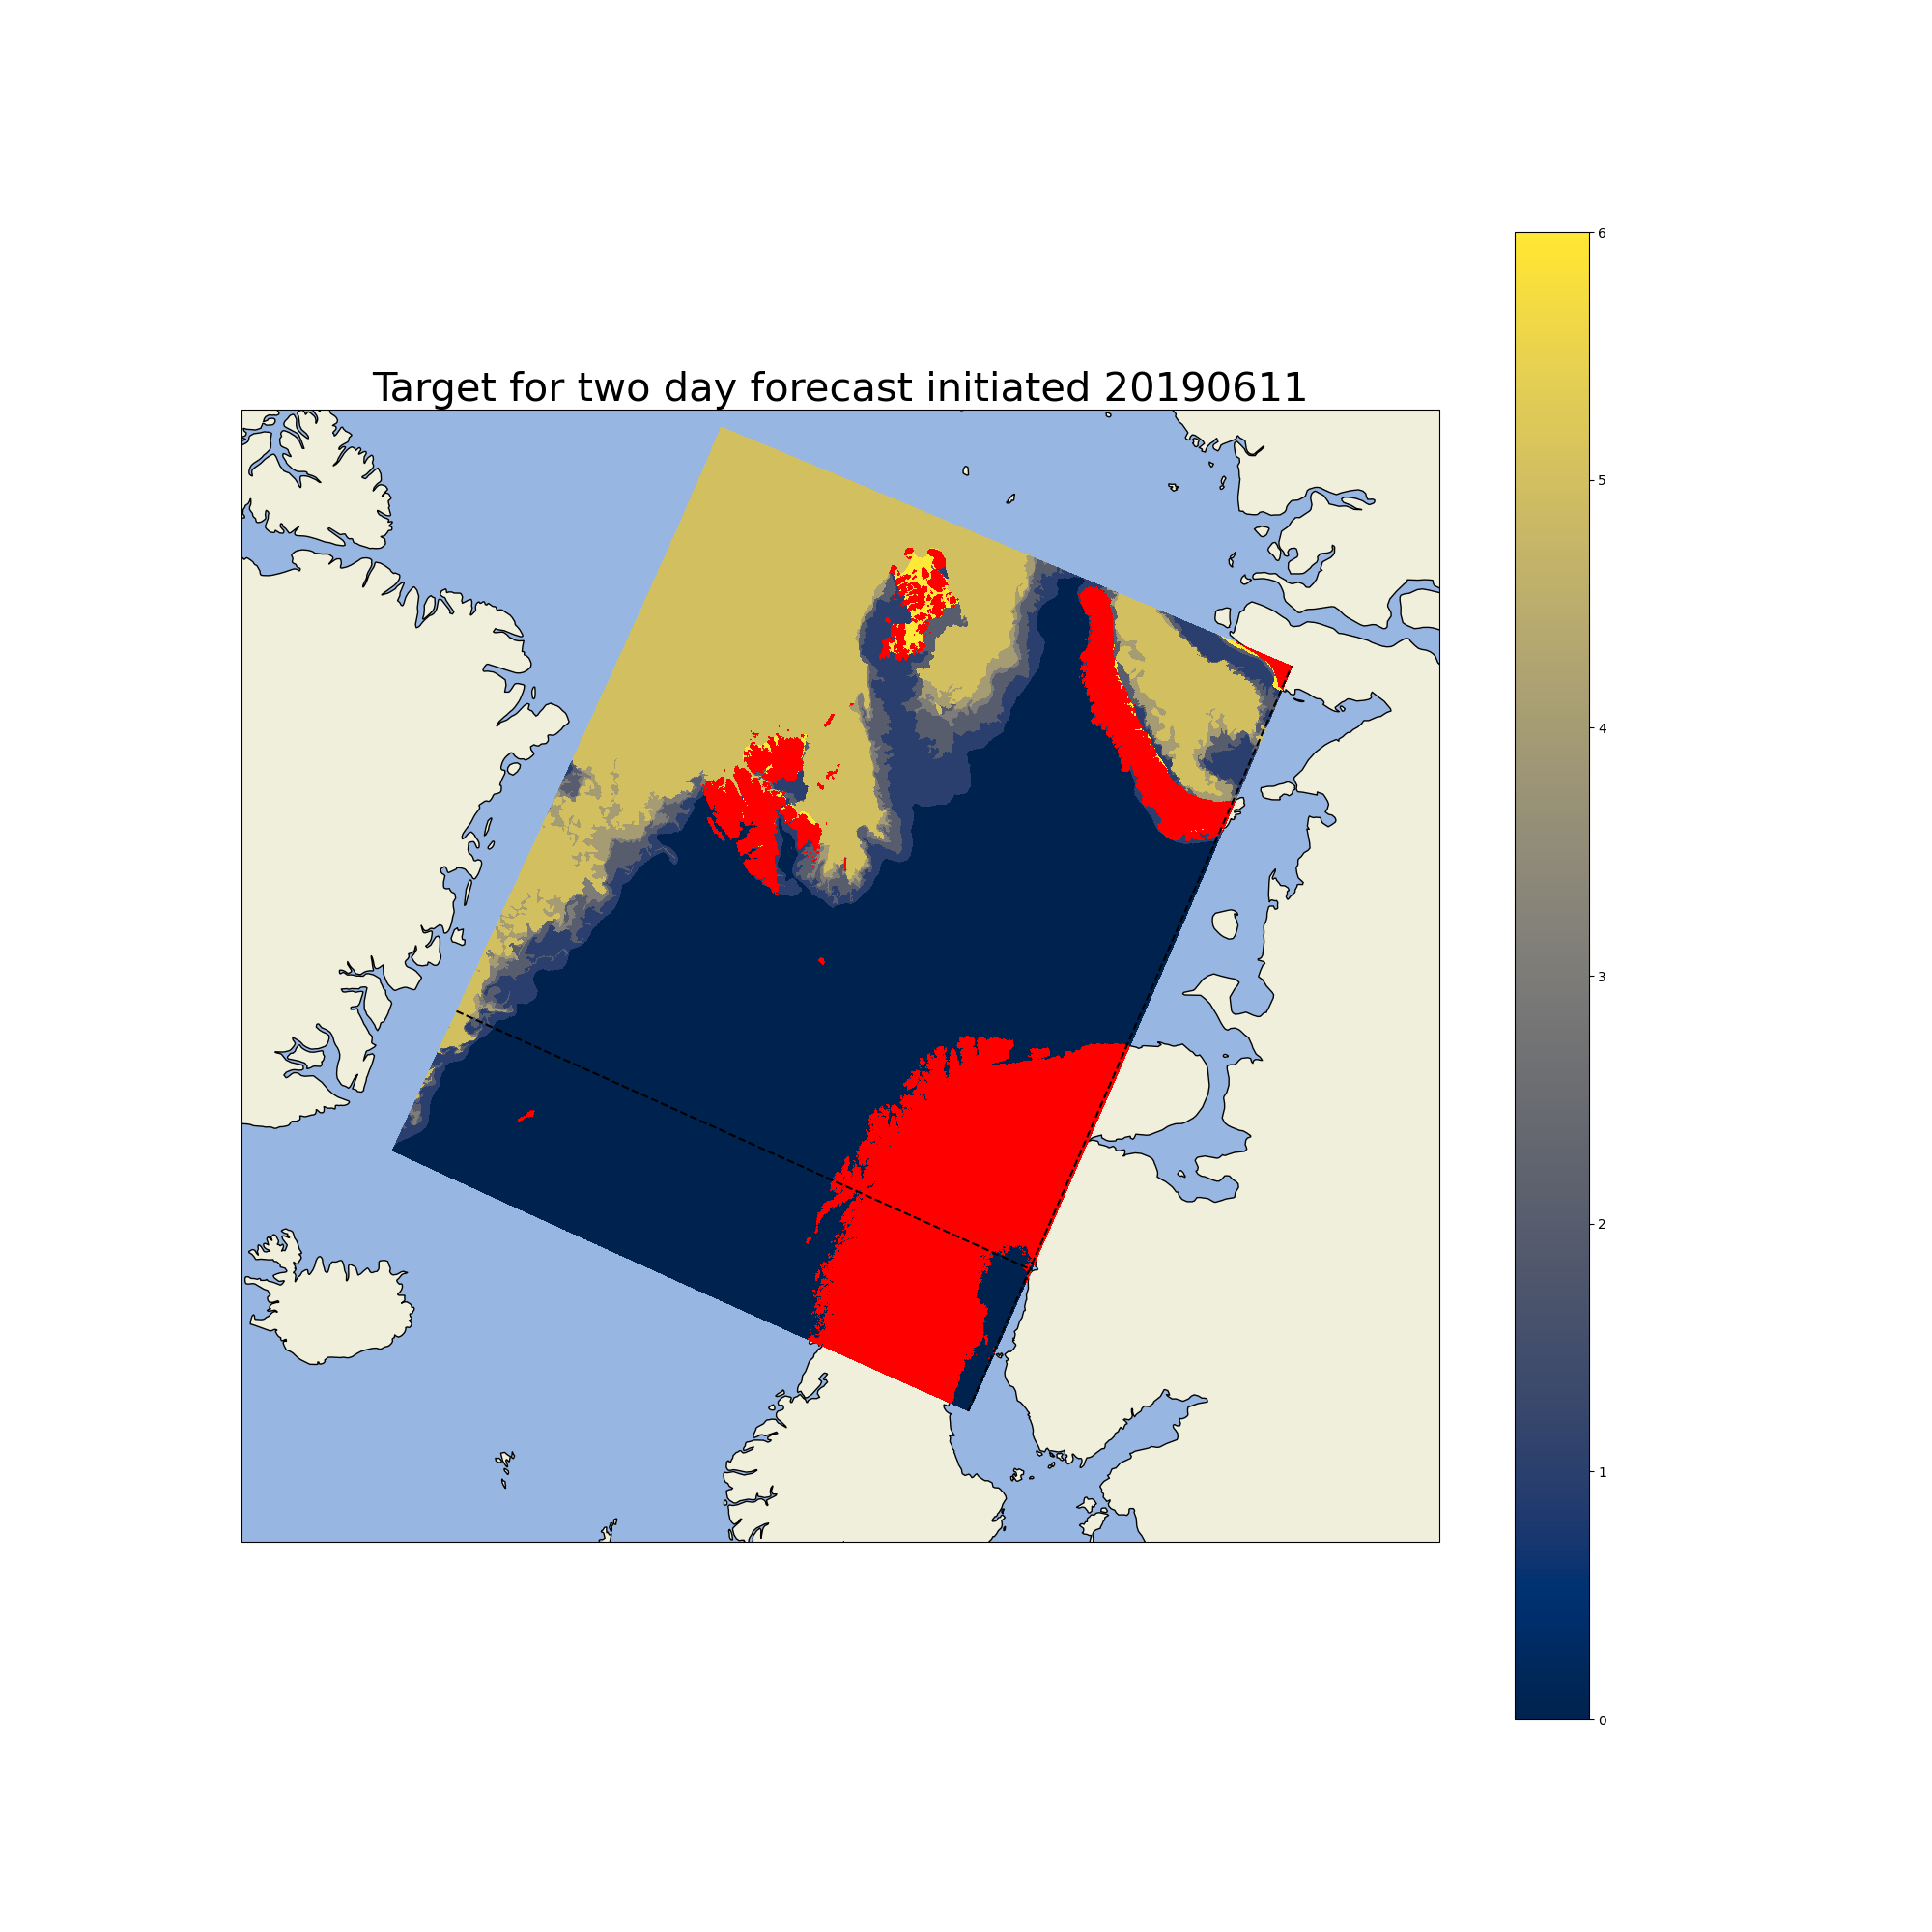
\includegraphics[trim={0 10cm 11cm 9cm}, clip, width=\textwidth]{20190611.png}
    \caption{\label{fig:exampleAAsouthborder}Example sample displaying an Ice Chart on a 1km Arome Arctic projection. Note the horizontal and vertical dashed black line which indicate the domain subsection used by the UNET}
\end{figure}

\section{Model Architecture}
The model architecture follows an encoder - decoder structure, commonly referred to as a U-NET \cite{Ronneberger2015} due to its shape funnelling the spatial data to coarser resolution, which resembles the letter "U". The current U-NET implementation follows that of Ronneberger et.al, though it has been modified with batch normalization after each convolution operation to ensure a more stable gradient flow. The weights of the model are Kaiming-He initialized \cite{He2015}, as the activation function used throughout the network is the ReLU function \cite{Nair2010}. The final output of the model is a (1920, 1840, 7) tensor containing softmaxed probabilities along its final axis.

\subsection{CategoricalCrossEntropy-Loss}
As the title suggests, these runs of the model involved using CategoricalCrossEntropy as the loss function for multi-class image segmentation. Categorical Cross Entropy loss is defined as 

\begin{equation}
    \label{eq:CE}
    CE = - \sum_i^C y_i\log{(\hat{y_i})}
\end{equation}

where $C$ denotes the number of available classes, $y$ the ground truth and $\hat{y}$ a prediction of $y$. Note that as $y$ is onehot-encoded, the formulated function only contributes to the overall loss with the log of the predicted probability of the correct class according to the ground truth.

Two variants of the previously described model have been trained with the CategoricalCrossEntropy described in equation (\ref{eq:CE}). The first model was trained with an encoder consisting of 4 convolutional blocks with channel dimensions (64, 128, 256, 512). The second model consisted of 5 convolutional blocks, with an identical architecture except for the last convolutional block increasing the channel dimension to (1024). Example outputs as well as target can be seen in Figure (\ref{fig:20210611}).

\begin{figure}
    \begin{subfigure}{0.49\textwidth}
        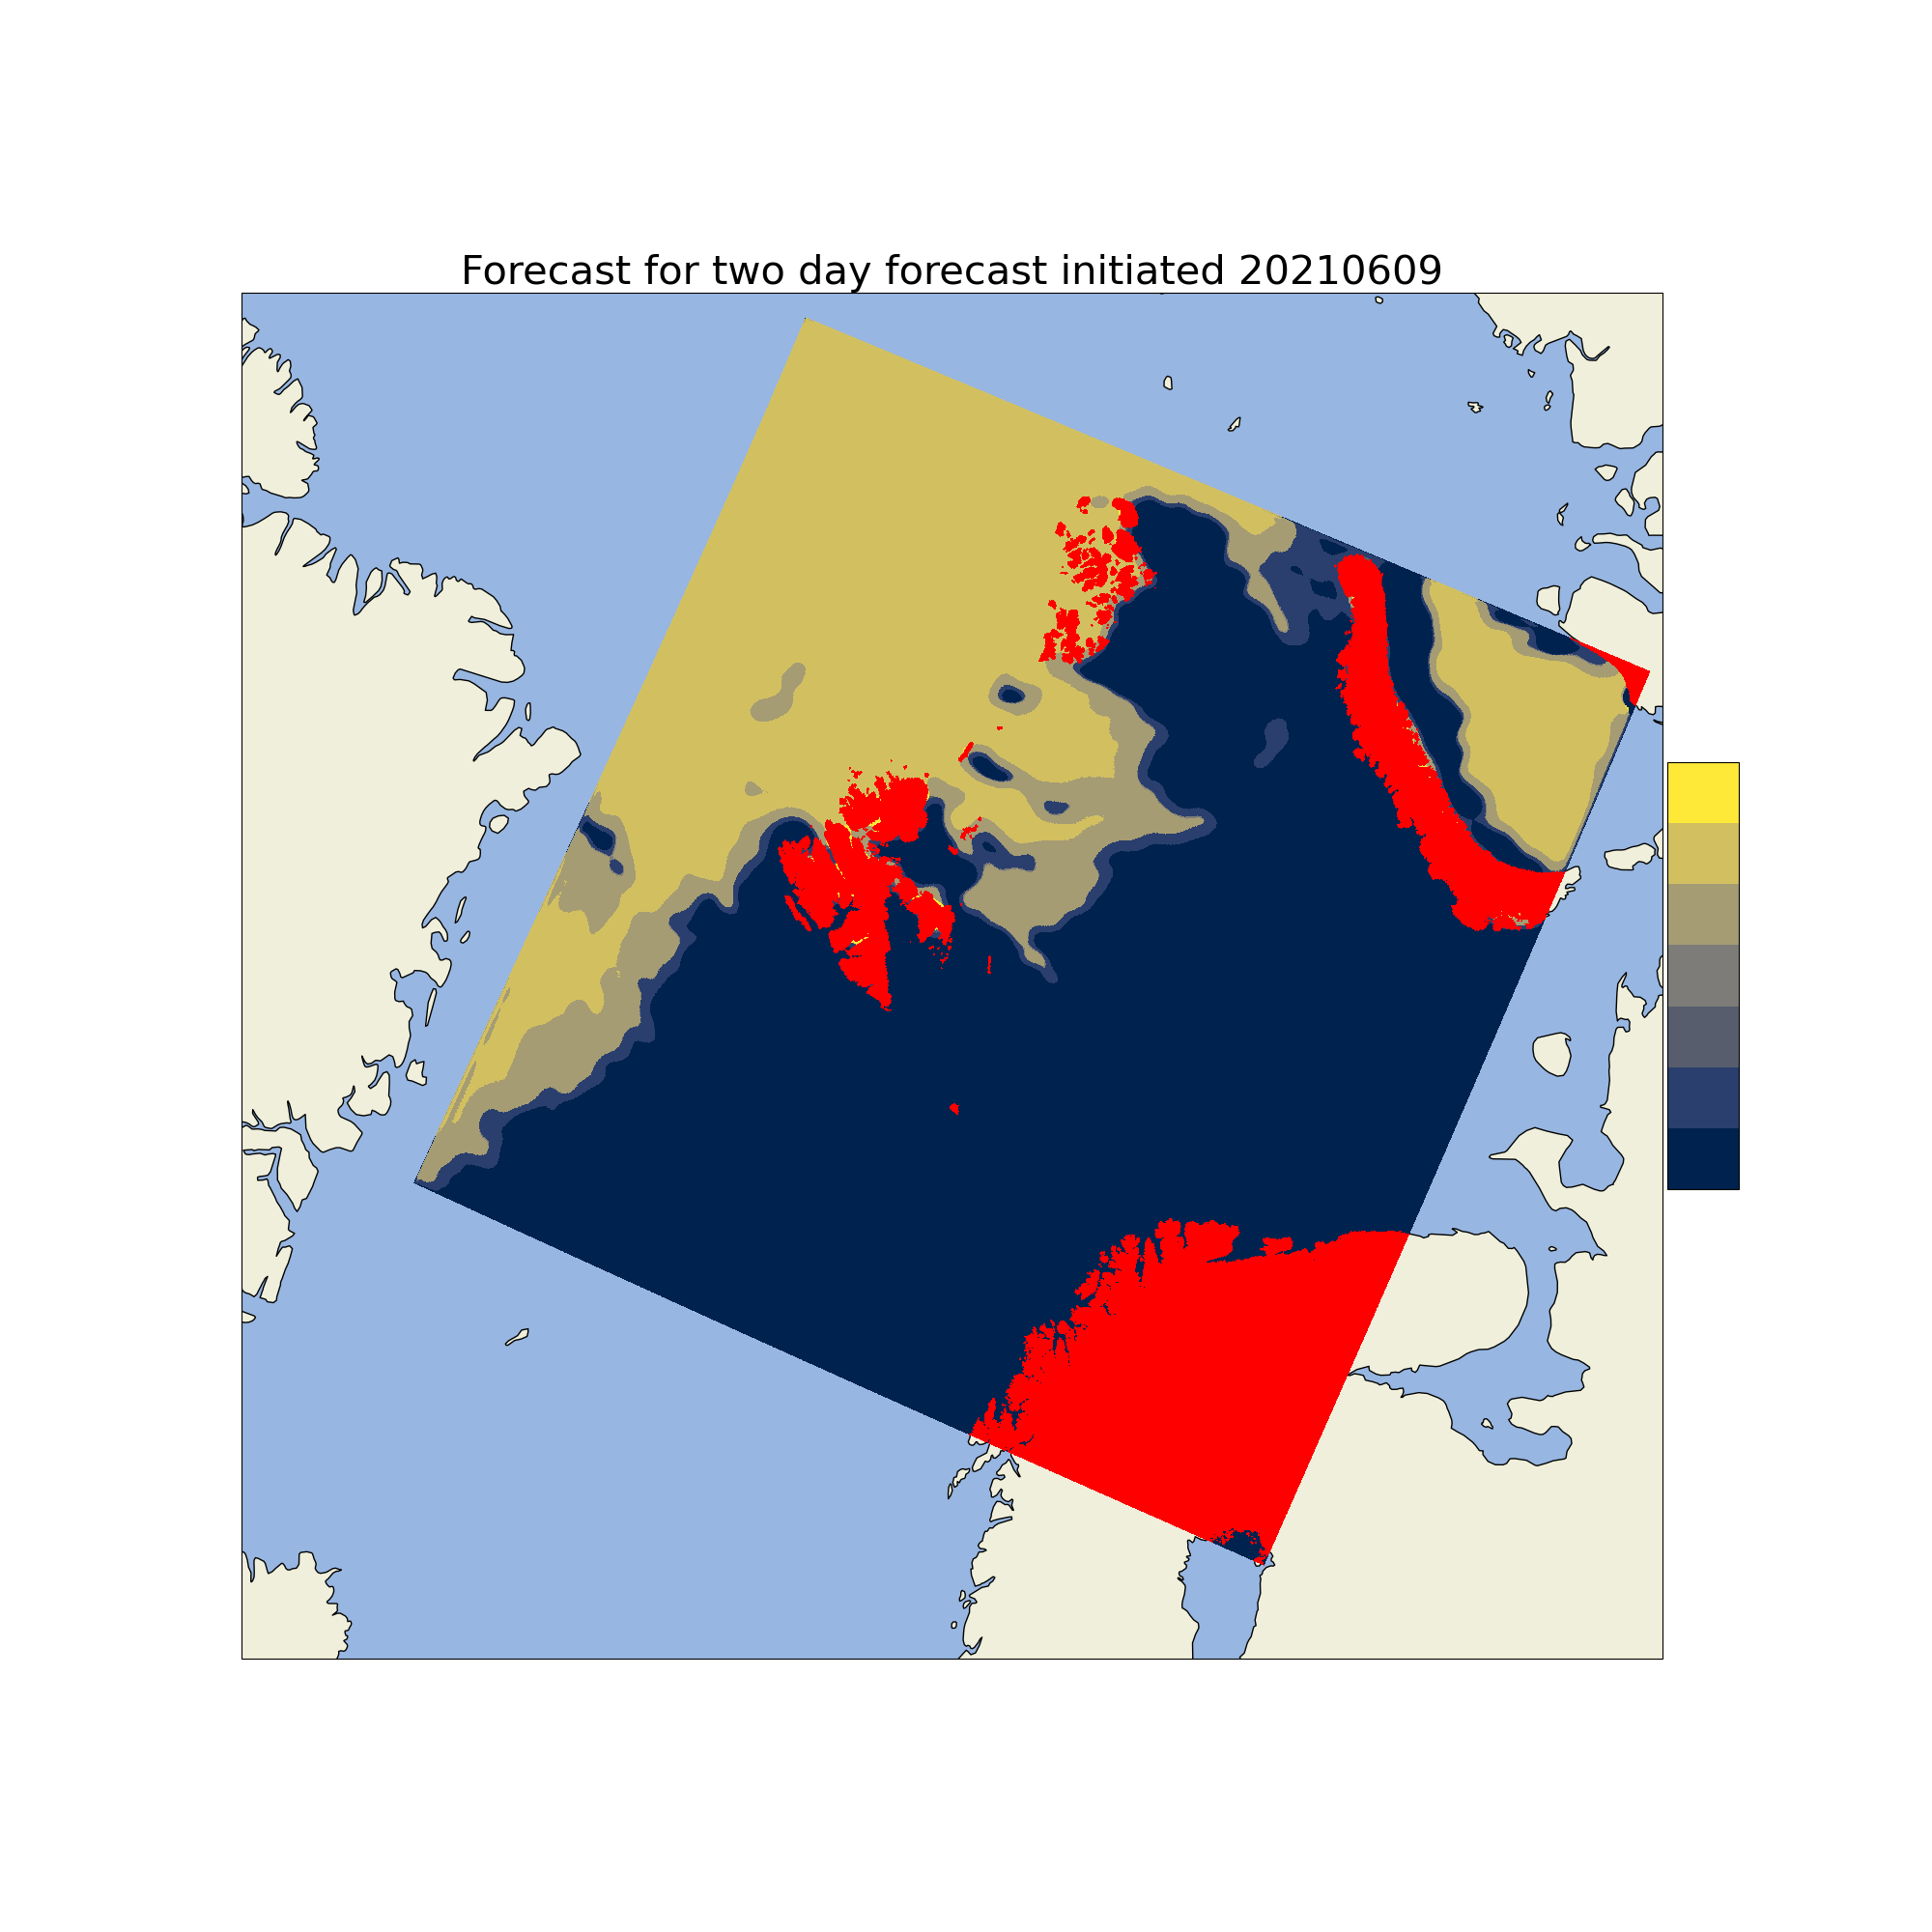
\includegraphics[width=\textwidth]{20210611_512.png}
        \caption{\label{fig:model51220210611}Forecast with two day lead time with model\_512 architecture}
    \end{subfigure}
    \hfill
    \begin{subfigure}{0.49\textwidth}
        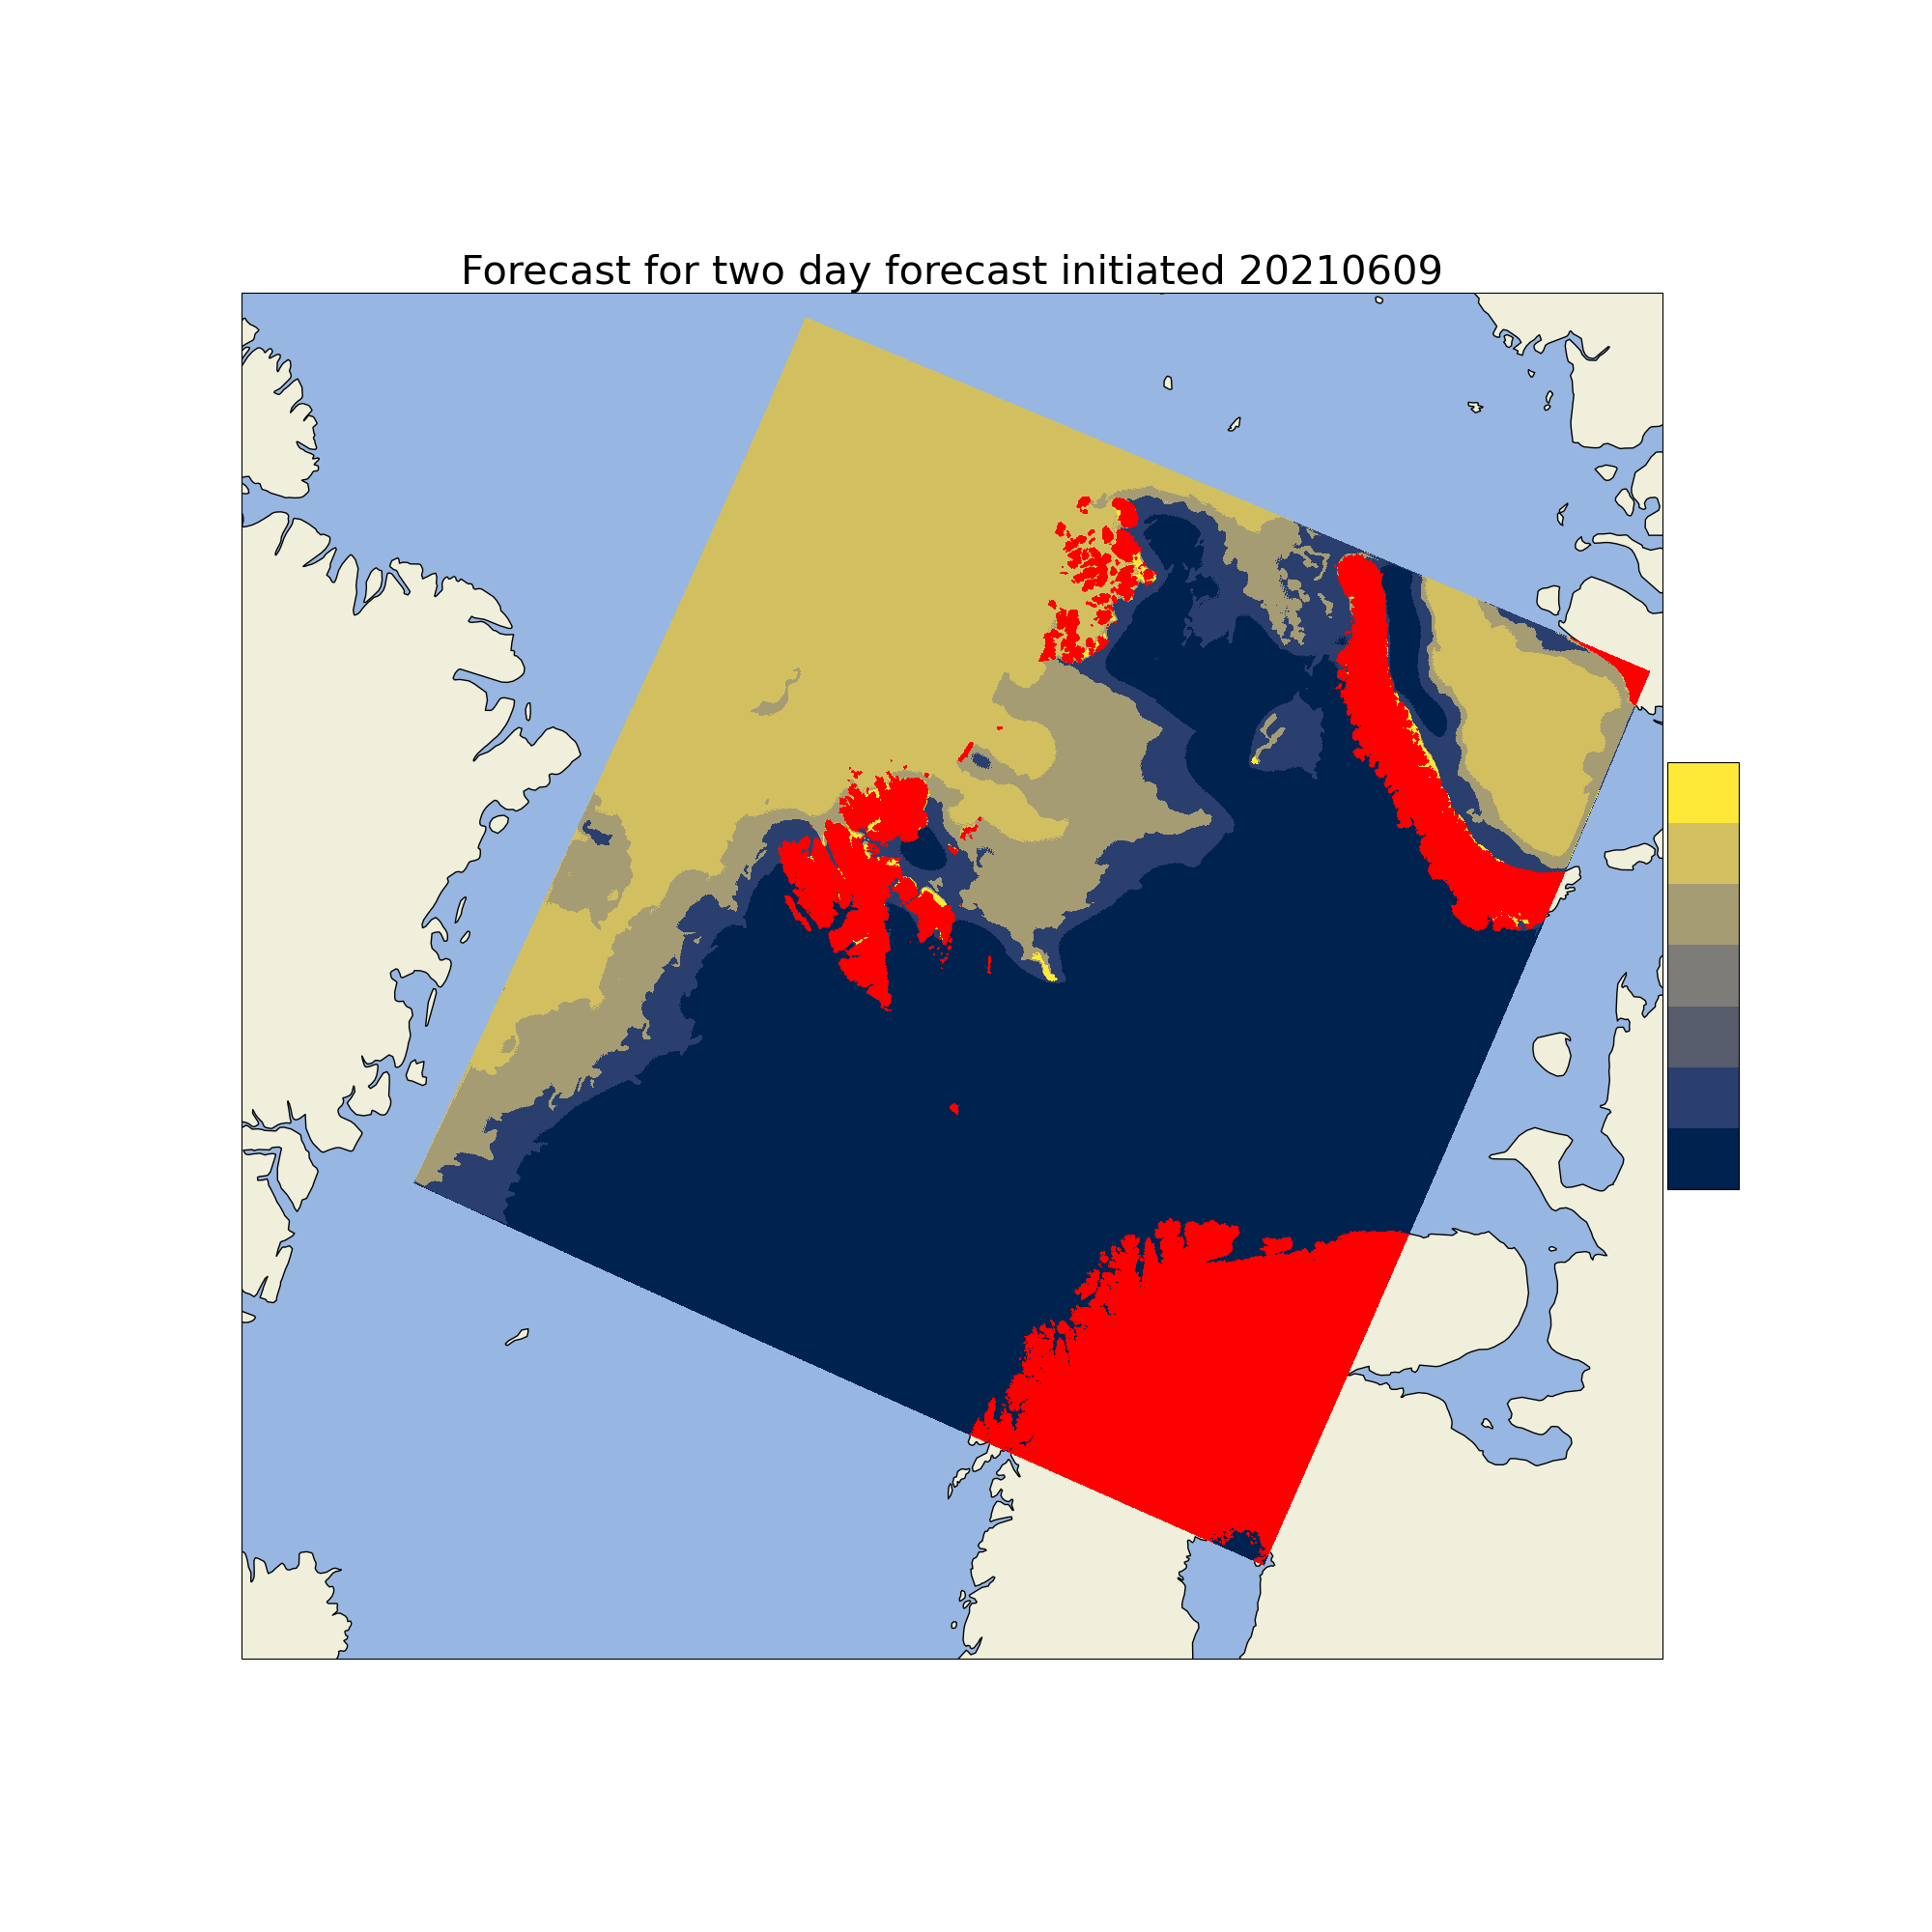
\includegraphics[width=\textwidth]{20210611_1024.png}
        \caption{\label{fig:model102420210611}Forecast with two day lead time with model\_1024 architecture}
    \end{subfigure}
    \begin{subfigure}{\textwidth}
        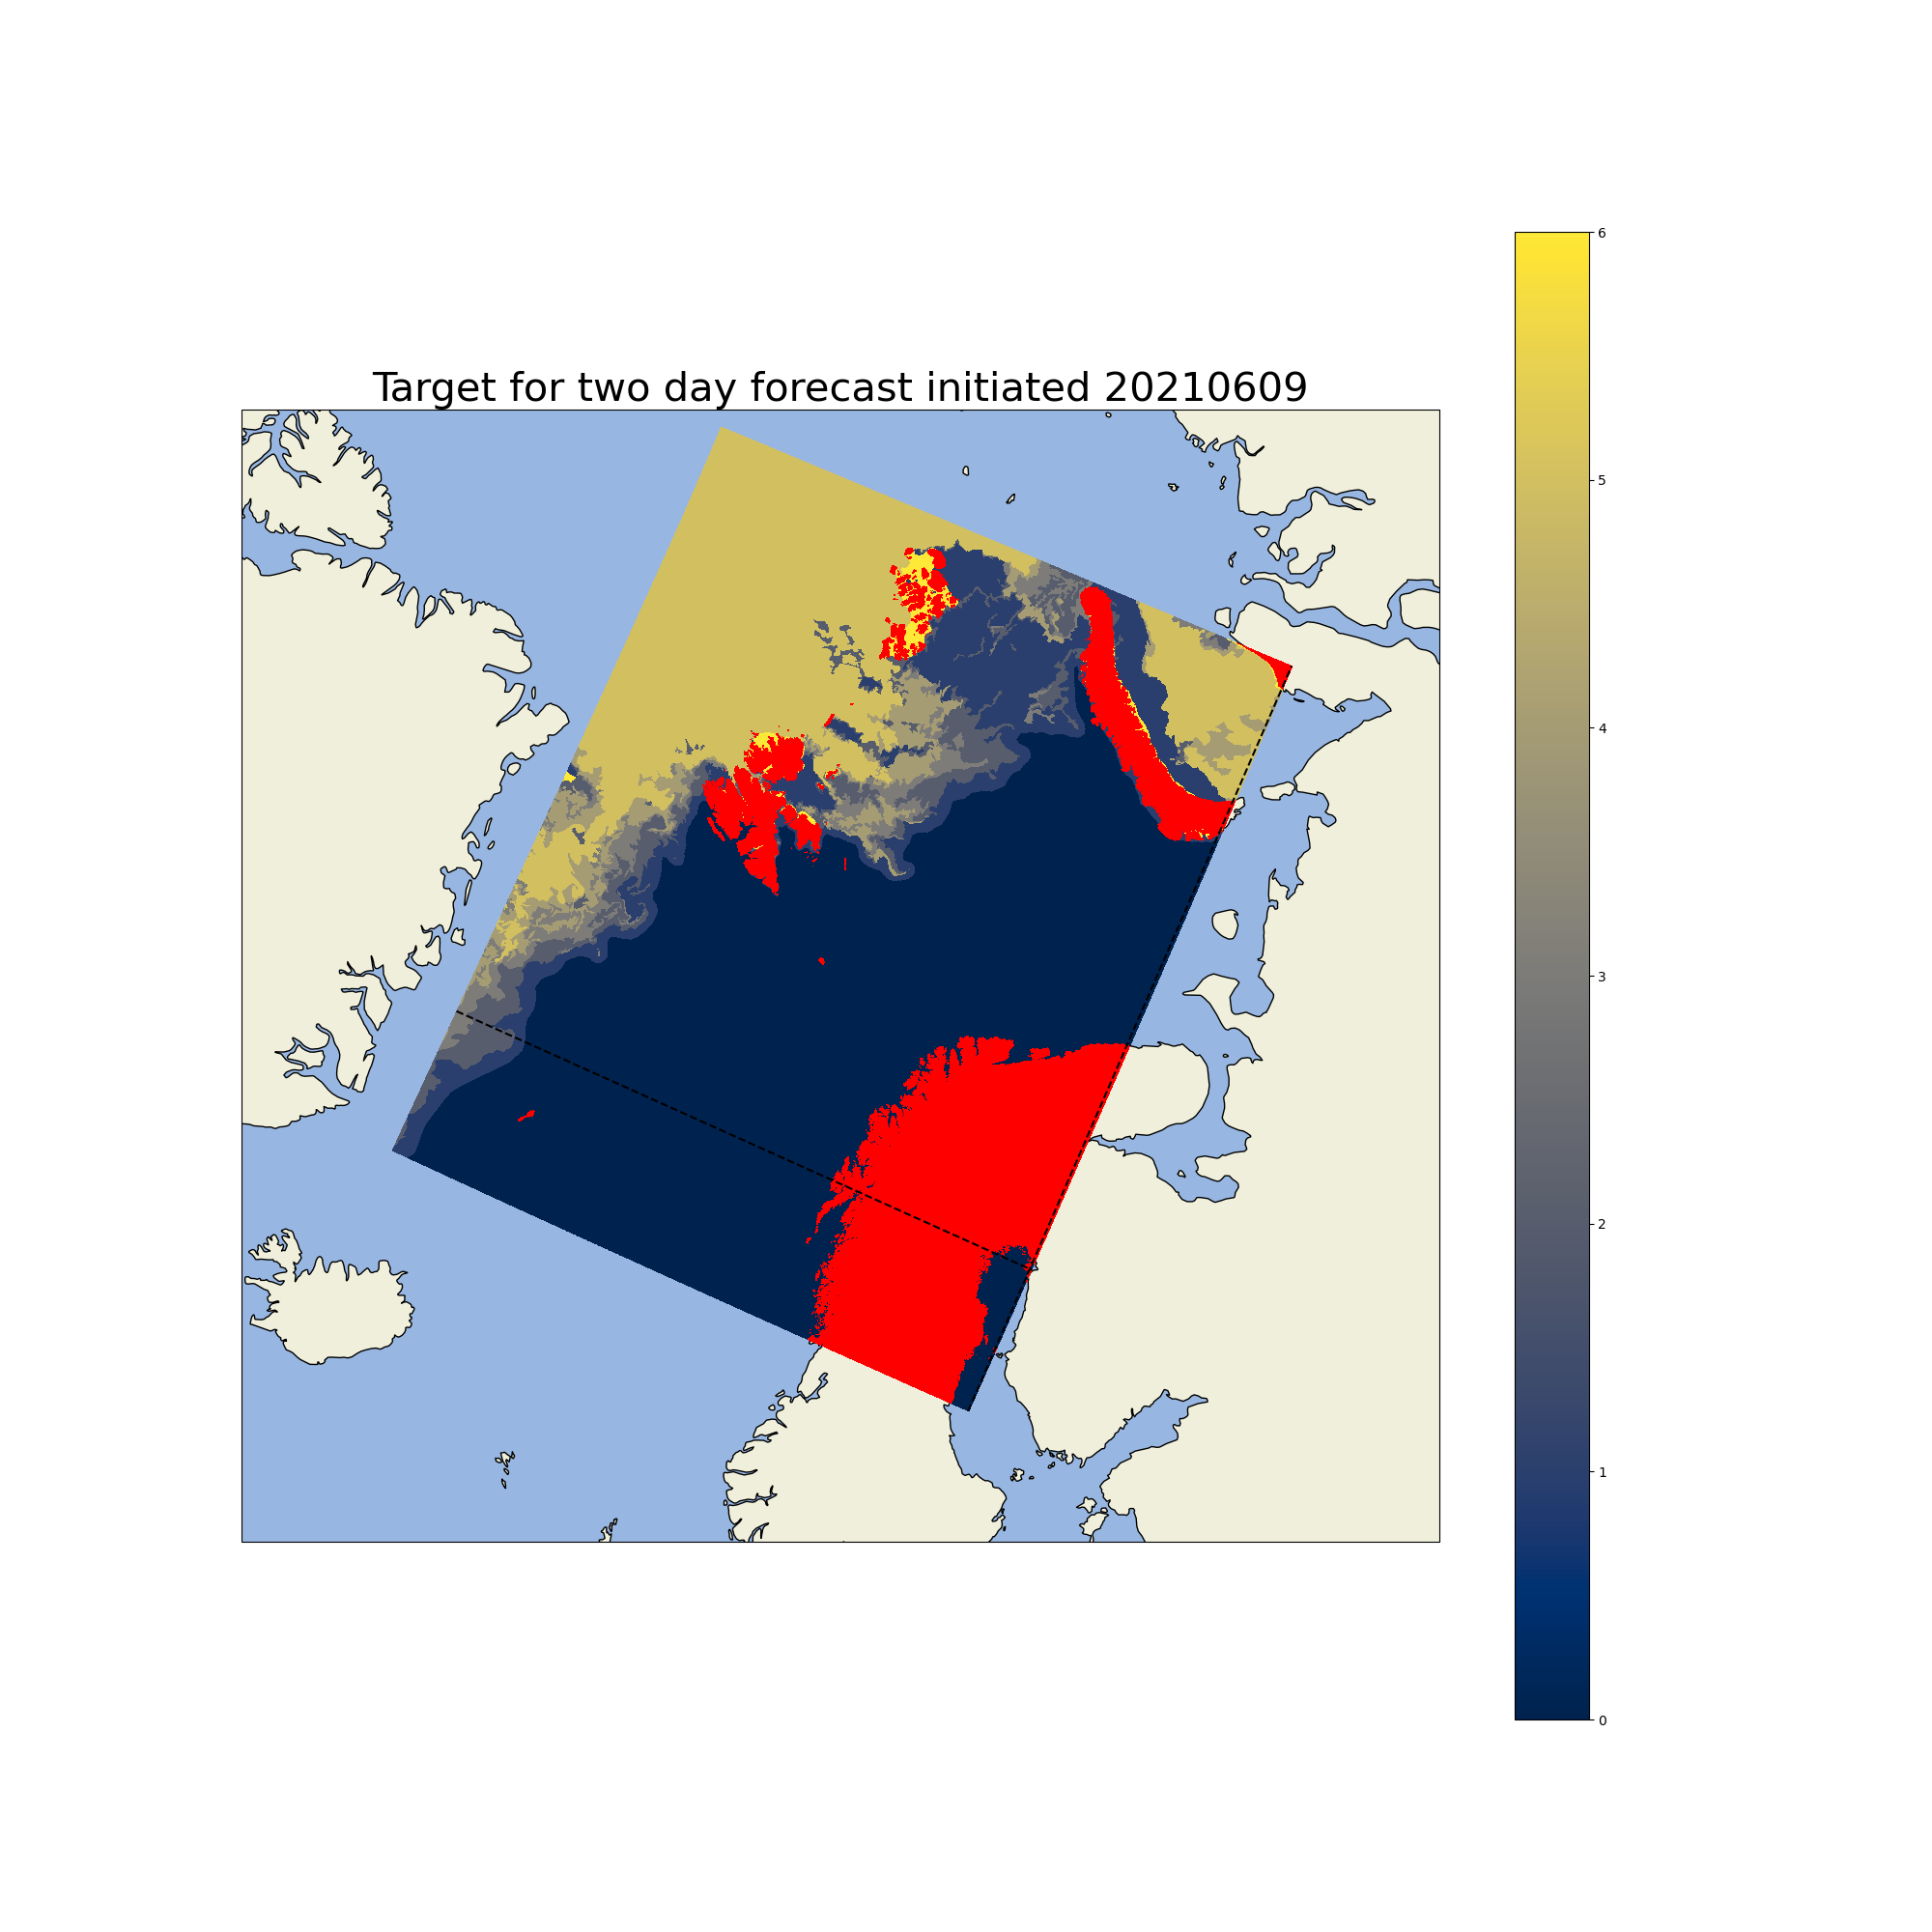
\includegraphics[trim={0 10cm 11cm 9cm}, clip, width=\textwidth]{20210611_target.png}
        \caption{\label{fig:target20210611}Target for forecast with two day lead time}
    \end{subfigure}
       \caption{\label{fig:20210611}Example forecast attempt made by model\_512 and model\_1024 09-06-2021}
\end{figure}

By inspecting Figure (\ref{fig:20210611}), two observations can be made. The first observation is regarding how the model complexity affects how it fit to the data. By comparing Figure (\ref{fig:model51220210611}) with (\ref{fig:model102420210611}), it can be seen that the latter is resolving the finer structures of the ice edge to larger extent than the prior. Though the overall correctness is left to be discovered, this shows that increasing the depth of the encoder (increasing the trainable parameter count from ~7 million to ~31 million) is reflected by the model preserving the details of the ice edge structure. Though it is non-trivial to say why the 1024-model preserves the details to a larger extent than the 512-model, it does follow from the U-Net architecture that a deeper encoder (higher channel count and more convolutional blocks) is better at describing "WHAT" is in the image compared to the shallow-layers, which include a larger amount of spatial information and tells the model to a larger extent "WHERE" things are in the model. \todo{This may have a source}

The second observation made from inspecting both forecasts is their inability to represent classes 2 and 3. This likely arises from the general movement-pattern of the sea ice, where the intermediate classes are much less likely to appear than the edge-most classes. Furthermore, the sea ice is much more likely to represent a wider range of concentration classes in the intermediate ice edge region over time, making it more difficult for the network to confidently predict those classes compared to the more probable classes. As can be seen by the network immediately predicting class 4 after class 1, creating an artificial cut-off region. However, to what extent the intermediate classes are predicted has not been inspected directly \todo{They should be}, though it is likely to assume that they are predicted though with a lower confidence than that of class 4 (which is consequently why it is visualized, as the most probable class is chosen regardless).



\subsection{FocalLoss}
\todo{Include figure showing focal loss output, discuss implications of using this loss function}
The focal loss is derived as a generalization of the Cross Entropy Loss listed in Equation (\ref{eq:CE}). The intent of the loss function is to downweight the easy to predict samples, while focusing on the hard to predict samples by allowing their gradient to have a higher impact on the network \cite{Lin2017}. Mathematically, focal loss is defined as

\begin{equation}
    \label{eq:FL}
    \text{FL} = -\sum_i^C\alpha_i(1 - \hat{y}_i)^\gamma y_i\log{(\hat{y}_i)}
\end{equation}

where $\alpha$ is a balancing parameter, $\gamma$ is the focusing parameter ($\gamma = 0 \rightarrow CE$), with the rest similar as Equation (\ref{eq:CE}).

By inspecting Equation (\ref{eq:FL}), it can be seen that predictions that the model is quite confident in making, i.e. $\hat{y}_i \rightarrow 1$ send the Focal Loss towards zero. For the current application, the assumptive motivation is that this affects (by reducing) the contribution made by the Ice Free Open Water pixels as well as the Very Close Drift Ice (class 6), which are the most represented classes in the CE loss model seen in Figure (\ref{fig:20210611}). Consequently, as the loss contributions of the most likely (and most represented classes) is reduced, the harder to predict (both due to being less represented and due to sea ice movement) have a larger impact on the overall loss propagating backwards throughout the model. As a result, these intermediate classes should be predicted as the most likely class, resulting in a less sharp ice edge which closer represent the Ice Charts. 


\subsection{Cumulative probability distribution model}
\todo{Discuss difference in dataloader, same dataset is used differently}

\subsubsection{Separate convolutionial layers as output}
\todo{Data exists, start writing}



\subsection{Model Selection}
During the training of a deep learning system, there exists several different ways to save a state of the model during training. A naive approach would be to let the model train all predetermined epochs, and save the weights of the model at the end of the final epoch. However, this approach would be indifferent to whether the model has converged, generalized or overfitted and is thus an inadequate way to save the weights. The Tensorflow Keras API supplies functions which can be used customize the training loop in the form of \href{https://www.tensorflow.org/api_docs/python/tf/keras/callbacks}{callbacks}, with the EarlyStopping and ModelCheckpoint callbacks relevant for model selection \cite{tensorflow2015-whitepaper}. EarlyStopping is a technique which ends the training loop when it detects that a monitored values has stopped decreasing. On the other hand, ModelCheckpoint continuously saves the model if a certain condition is met, without terminating the training loop. Both callbacks support monitoring the validation loss as the metric in which to optimize the model. However, a custom metric such as yearly mean IIEE \cite{Goessling2016} could be monitored instead. 

To aid in model selection, I developed a custom callback which computed the Normalized IIEE with respect to a climatological Ice Edge length derived from ten years of OsiSaf data \todo{Write about the climatological Ice Edge dataset, ref section from here}, following the observation in \ref{sec:Impact of increased resolution on the IIEE} that IIEE is correlated across spatial resolutions. The callback computes said metric for all samples and reduces them to a yearly mean of the validation set. Similar to the aforementioned callbacks, the developed callback is executed at the end of an epoch where it computes the mean Normalized IIEE for all predicted samples from the validation set, which it appends to the \textit{logs} dictionary used by Tensorflow to keep track of other computed metrics, such as loss and validation\_loss for the current case. Thus, the newly developed callback would allow for model selection based on Normalized IIEE, as well as the already computed validation loss.

When comparing different models to asses their performance, this project will frequently compare their Normalized IIEE as the metric is Normalized by the ice edge, thus reducing the seasonal variability of the Metric \cite{Palerme2019} \todo{This citation is actually for $\text{SPS}_\text{length}$ but SPS is reduced to IIEE for a deterministic ice edge \cite{Goessling2018}}. As such, it would be beneficial to select a model based on its Normalized IIEE validation performance. With the above callback, such a selection is possible. However, including the IIEE verification metric as is done in the above callback increases training-time of ten epochs from $\approx$ two hours without the IIEE callback to $\approx$ 24 hours with the IIEE callback. As 20 epochs is currently an adequate number of epochs at the time of writing \todo{This may change}, it would be too computationally costly to select a model based in its validation Normalized IIEE performance. 

\begin{figure}
    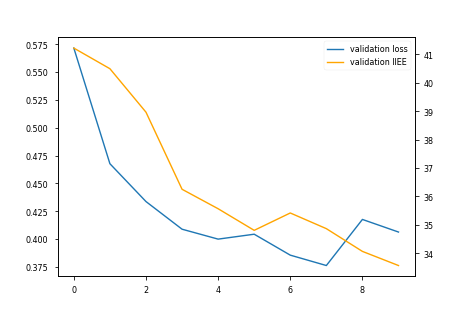
\includegraphics{val_loss_IIEE.png}
    \caption{\label{fig:val_loss_iiee_corr}validation loss and Normalized IIEE computed as mean of validation set for each epoch during training}
\end{figure}\todo{tmp figure, redo with inspect data notebook in ForecastVerification}
On the other hand, it can be seen by inspecting Figure (\ref{fig:val_loss_iiee_corr}) that the Normalized IIEE tend to evolve conjunctionally with the validation loss, in the current case defined as the mean cross entropy of all validation samples. Furthermore, the validation loss and Normalized IIEE in Figure (\ref{fig:val_loss_iiee_corr}) have a correlation of $0.82$ with regards to epoch. Note that this has been calculated only using the numbers present in Figure (\ref{fig:val_loss_iiee_corr}). As such, there is reason to believe that selecting a model based on its validation loss, which is quick to compute, would result in a generalized model which may also excel at lowering its Normalized IIEE.

When selecting the best model, this project will apply the ModelCheckpoint callback with regards to validation loss as outlined above. ModelCheckpoint is preferred compared to EarlyStopping, as interrupting the training loop early may result in an "undercooked" model. E.g. the weights in earlier model layers are adjusting slower than later weights, giving the impression that the model training has reached a plateau which causes the model to stop. Whereas if the model where to continue training, the later adjustment of earlier weights would cause a later spur in increased model performance. ModelCheckpoint was chosen since behavior such as what was just exemplified is possible with the callback.

[Training and validating a deep learning system requires data, which can be categorized in two distinct groups. The first group is the data known by the system, which is used during training to increase or validate model performance. Additional to the data used during training is external data, which is needed to validate the generalizability of the model. I.e., how well does the model perform with unknown data, which is assumed to be drawn from the same distribution as the data used during training. It is standard practice to arbitrarily split by a given fraction into the three datasets (training, validation, testing), as outlined above. However, due to the variable seasonal dependency of meteorological data, a naive split of the data could result in seasonally unbalanced datasets. As such, the datasets constructed for this thesis's purpose cover at least a full year. Thus, no dataset is assumed to be skewed in the direction of any season.] \todo{Dette passer bedre inn i en train-test-split \textbf{model development}}

\biblio
\end{document}